\documentclass[12pt]{report}
\usepackage[utf8]{inputenc}
\usepackage{amsmath}
\usepackage{theorem}
\usepackage{geometry}
\usepackage{hyperref}
\usepackage{graphicx}
\usepackage{amsfonts}
\usepackage{tabularx}
\usepackage{algorithm}
\usepackage{algpseudocode}


\newtheorem{definition}{Definition}
\newtheorem{notation}{Notation}
\newtheorem{claim}{Claim}
\newtheorem{case}{Case}

\geometry{bottom=30mm, top=30mm, left=30mm, right=30mm}

\title{
    \textbf{\Huge{Theory Assignment 3}} \\
    \vspace*{15pt}
    \large{CSE222: \textit{Algorithm Design \& Analysis}}
}

\author{
    \href{mailto:divyajeet21529@iiitd.ac.in}{Divyajeet Singh (2021529)}
}

\date{
    \vspace*{10pt}
    \textbf{\today}
}

\graphicspath{{./Assets/}}


\begin{document}
    \maketitle

    \section*{\huge{Problem}}
    The towns and villages of the Island of Sunland are connected by an extensive rail network.
    Doweltown is the capital of Sunland. Due to a deadly contagious disease,
    a few casualties have been reported in the village of Tinkmoth. To prevent the disease from
    spreading to Doweltown, the Ministry of Railway of Sunland wants to completely
    cut down the rail communication between Tinkmoth and Doweltown. \\
    For this, they wanted to put traffic blocks between pairs of stations, $x$ and $y$, that are
    directly connected by a railway line (i.e., there are no stations between them on that line).
    If a traffic block is put in between $x$ and $y$, then no train can travel from $x$ to $y$ from that
    line. To minimize expense (and public notice), the authority wants to put as few traffic blocks
    as possible. \\
    Formulate the above as a flow-network problem and design a polynomial-time algorithm to
    solve it. Give a precise justification of the running time of your algorithm.

    \subsection*{Input}
    An graph $G = (V, E)$ representing the layout\footnote{
        We assume that Tinkmoth and Doweltown have two distinct railway stations, $v_{t}, v_{d} \in V$.
    } of the island, along with $v_{t}$ and $v_{d} \in V$, the railway stations of Tinkmoth and Doweltown. \\
    $V$ is the set of all railway stations and $E$ is the set of all railway lines in Sunland.
    \vspace*{7.5pt} \\
    \textbf{Note:} \textit{Formulation of the problem as a flow-network problem is given in the subsequent subsection.}

    \subsection*{Output}
    The minimum number of traffic blocks to be installed to cut down the rail communication between Tinkmoth and Doweltown.

    \subsection*{Solution}
    The given problem can be solved using the concept of minimum cut in a flow-network.
    A minimum cut in a flow-network is a minimal set of edges whose removal disconnects the source vertex from the sink.
    Since we are required to find the minimum number of traffic blocks required to disconnect the railway network between Tinkmoth and Doweltown,
    we can find the number of edges in a minimum cut of $G$.
    The following sections discuss the apporach to solve the problem in detail.

    \subsubsection*{Notations Used}
    \begin{notation}[$f(u \to v)$]
        The flow through the edge $(u \to v) \in E$.
    \end{notation}
    \vfill

    \subsubsection*{Formulation as a flow-network problem}
    Since this problem deals with the railway network of a city, it can be naturally solved using graphs.
    Each station on the Island can be considered as a vertex $v \in V$.
    The railway lines connecting pairs of stations $u$ and $v$, can be considered as two directed edges $(u \to v) \in E$ and $(v \to u) \in E$. \\
    Since the Ministry of Railway intends to stop the spread of infection from Tinkmoth to Doweltown, $v_{t}$ and $v_{d}$
    can be considered as the source and the sink respectively.
    Finally, the problem can be converted to a flow-network by assigning a capacity $c(u \to v)$ to each edge $(u \to v) \in E$ as follows:
    \begin{equation}
        \label{eq:capacity}
        c(u \to v) = \begin{cases}
            0 & \text{ if $u = v_{d}$ or $v = v_{t}$} \\
            1 & \text{ otherwise}
        \end{cases}
    \end{equation}
    For each edge $(u \to v_{t})$, $c(u \to v_{t}) = 0$ signifies that $v_{t}$ is the source and no flow can enter it.
    Similarly, $c(v_{d} \to w) = 0 \ \forall \ (v_{d} \to w) \in E$ as $v_{d}$ is the sink and no flow can exit it.
    The capacity of all other edges is 1 as we can cut down communication between two stations using only one traffic block. \\
    In this manner, we create a flow-network $G = (V, E)$ with $v_{t}$ as the source and $v_{d}$ as the sink, based on the island's railway network. \hfill
    \begin{figure}[htp]
        \begin{center}
            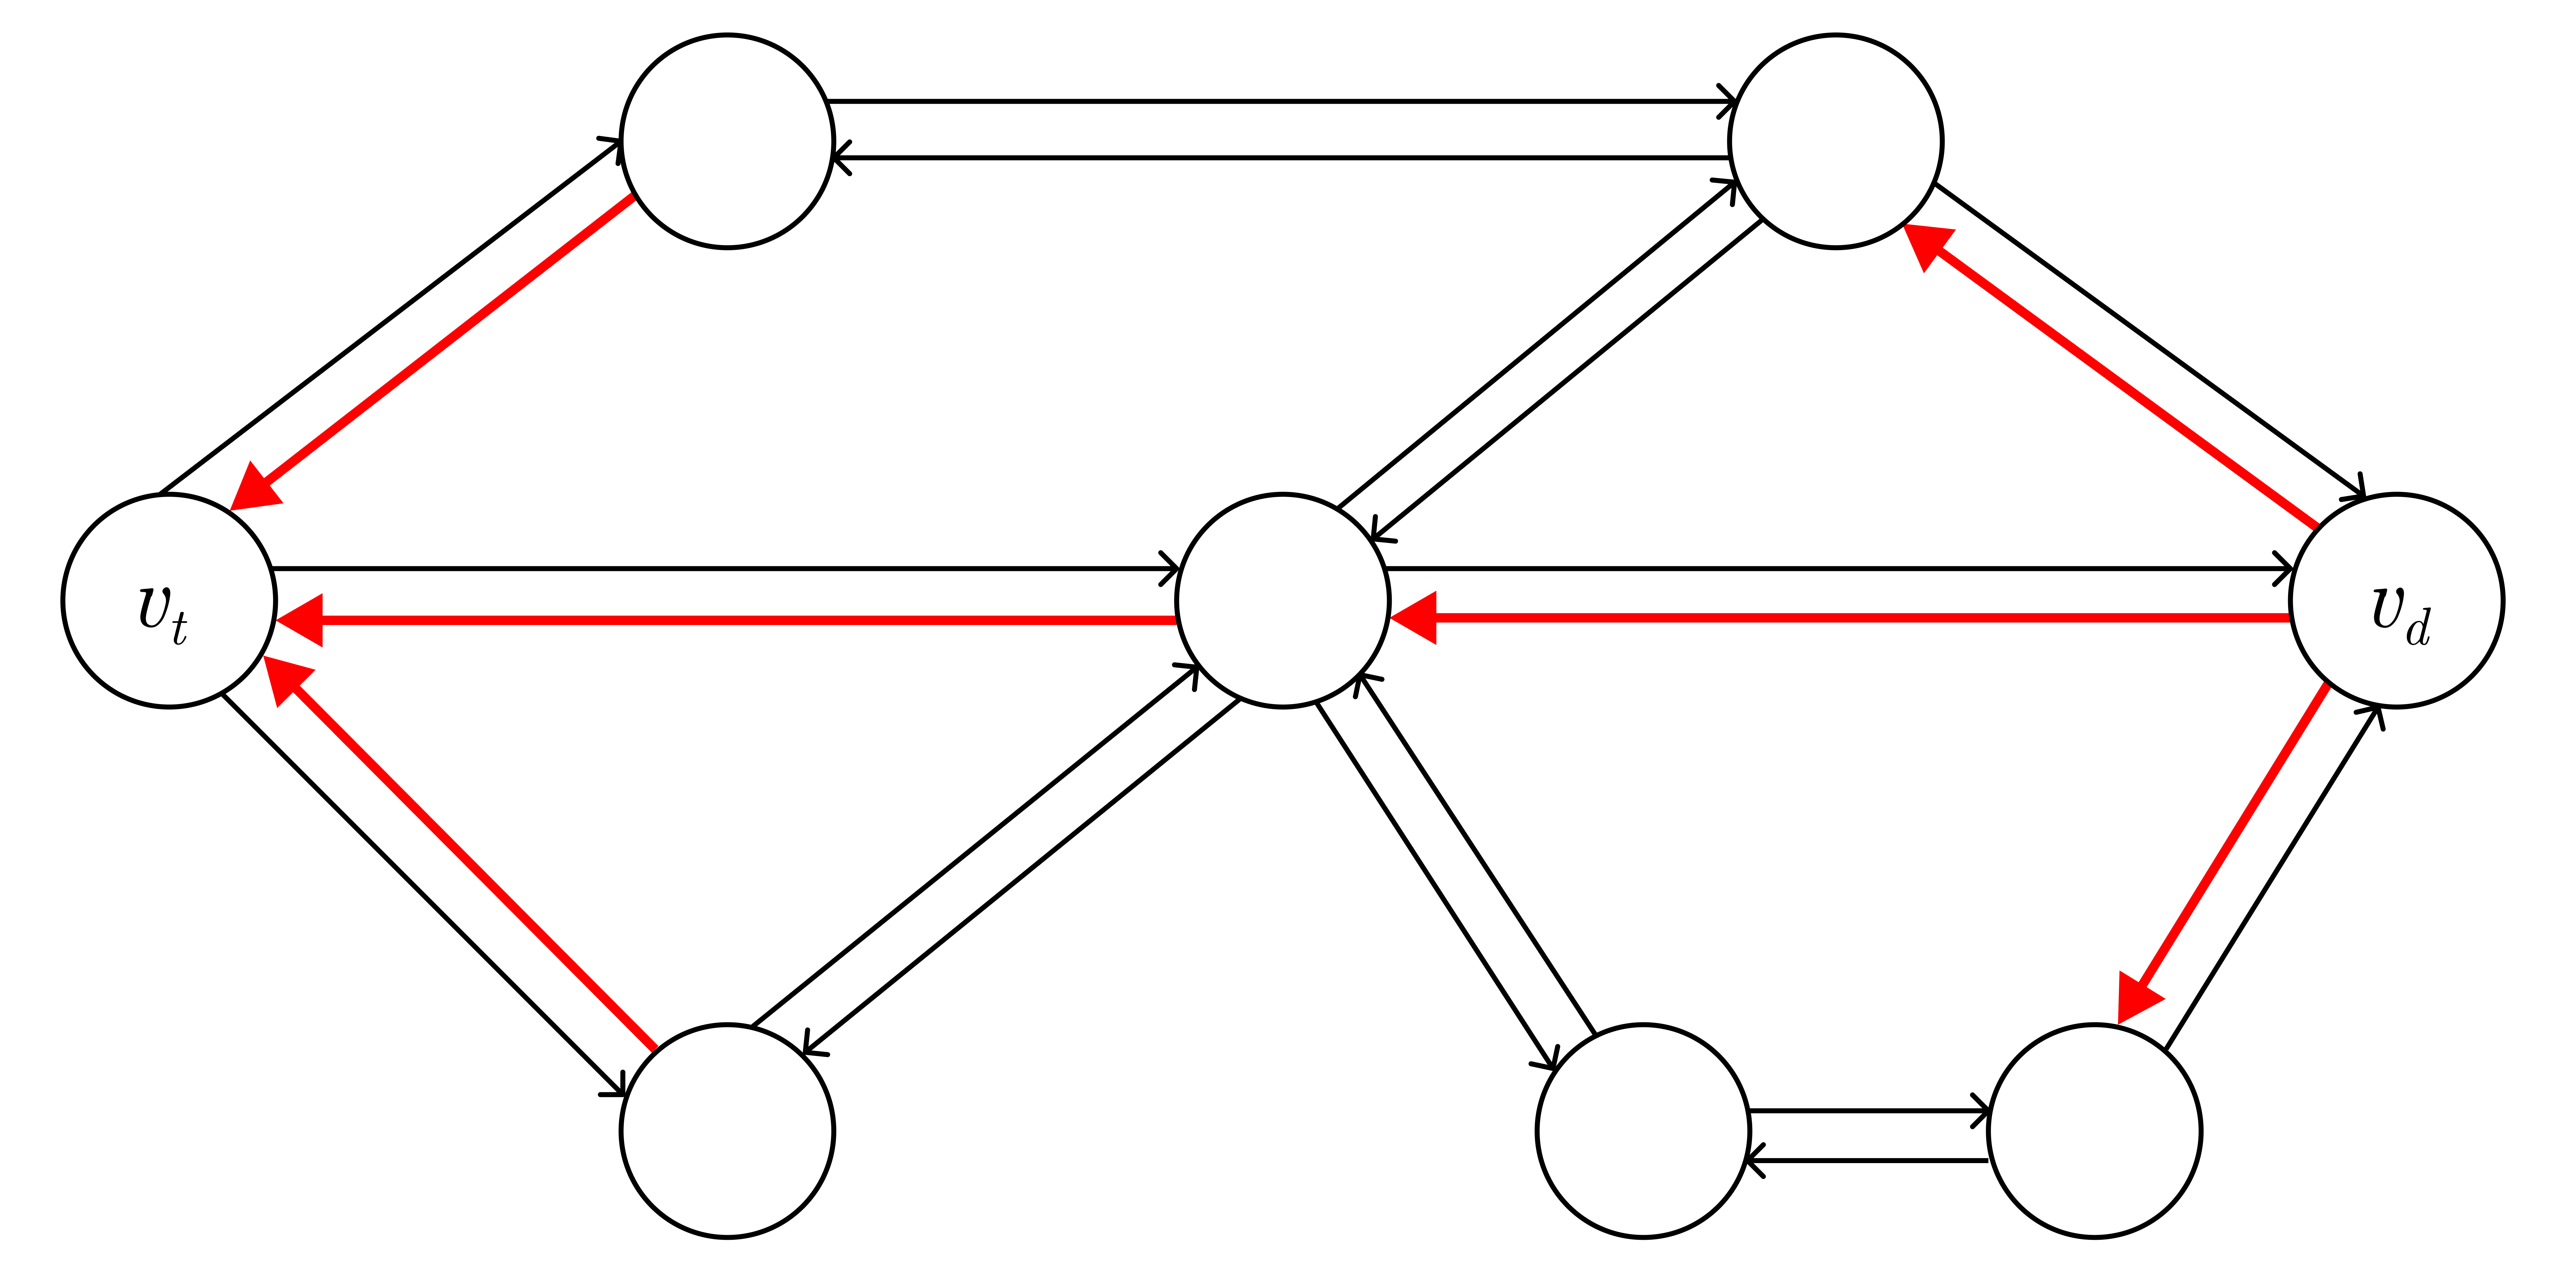
\includegraphics[width=0.7\textwidth]{network.png}
        \end{center}
        \caption{An example flow-network $G$ for the Island of Sunland.}
        \label{fig:network}
    \end{figure}
    \vspace*{10pt} \linebreak
    Figure (\ref{fig:network}) shows a rough diagram depicting the flow-network $G$ for the Island of Sunland.
    Here, the red edges have a capacity of 0 and the rest have a capacity of 1.
    This construction ensures that in the beginning, no flow can enter the source $v_{t}$ and no flow can exit the sink $v_{d}$.
    \vspace*{10pt} \\
    \textbf{Note:} \textit{Since flow is always calculated using simple paths, the maximum flow is actually independent of the initial capacities of the red edges.
    This is because including them in any $v_{t}-v_{d}$ path would produce a cycle.
    However, for the sake of argument, setting their capacities to 0 ensures that $v_{t}$ and $v_{d}$ behave as the source and the sink, even visibly.}

    \subsubsection*{The Solution Description}
    The problem can be solved by using the Ford-Fulkerson Algorithm\footnote{
        Ford-Fulkerson Algorithm was discussed in Lecture-17 of the course \textbf{CSE222} by \href{mailto:debarka@iiitd.ac.in}{Dr Debarka Sengupta},
        Winter 2023.
    } to find the maximum flow of the flow-network.
    In our case, the maximum flow of the flow-network gives the maximum
    number of \textit{paths} through which the disease can spread from the source to the sink.

    \begin{claim}
        \label{claim:max-flow-min-cut}
        The maximum flow $f^{*}$ of the flow-network $G$ is equal $n^{*}$, to the minimum number of traffic blocks to be installed to cut down the
        rail communication between Tinkmoth and Doweltown.
    \end{claim}
    \textit{Proof.}
    \begin{quote}
        By assignment (\ref{eq:capacity}), $f^{*}$ is equal to the number of simple paths from $v_{t}$ to $v_{d}$ that can be traversed \textit{simultaneously} in $G$.
        This is because any edge $(u \to v)$ with $f(u \to v) = 1$ is already at its bottle-neck, and cannot be used to traverse any other path. \\
        Each traffic block blocks one path, as an already used/blocked line cannot be involved in another path. So, there are exactly $n^{*}$ simple
        paths from $v_{t}$ to $v_{d}$ in $G$. \\
        Hence, $f^{*} = n^{*}$. \hfill $\square$
    \end{quote}
    However, the Ford-Fulkerson Algorithm runs in pseudo-polynomial time, as it is a multiplicative of the maximum flow of the network,
    which can be arbitrarily large (exponential in the input size).
    Hence, to solve the given problem in polynomial time, we make the following (very crucial) claim.

    \begin{claim}
        \label{claim:polynomial}
        The maximum flow of a flow-network is linear in the number of vertices when
        the capacities are assigned as described in (\ref{eq:capacity}).
    \end{claim}
    \textit{Proof.}
    \begin{quote}
        Let $G = (V, E)$ be a flow-network with a source $v_{t}$ and a sink $v_{d}$, with maximum flow $f^{*}$.
        Assume that capacities assigned to all edges in $E$ as described in (\ref{eq:capacity}).
        \vspace*{10pt} \\
        Then, $f^{*}$ in $G$ is bounded above by $|V_{t}|$, where $V_{t}$ is the set of vertices connected to $v_{t}$.
        This is because, at best, only as much flow can reach the sink as much leaves the source.
        \begin{equation}
            f^{*} \leq \sum_{w \in V_{t}} f(v_{t} \to w) \leq \sum_{w \in V_{t}} c(v_{t} \to w) = \sum_{w \in V_{t}} 1 = |V_{t}| \leq |V|
        \end{equation}
        Hence, $f^{*} \leq |V_{t}| \leq |V| \implies f^{*} = O(|V|)$. \hfill $\square$
    \end{quote}
    \vfill
    The above claim is key to solving the problem in polynomial time.
    As a by-product of claim (\ref{claim:polynomial}), the Ford-Fulkerson Algorithm runs in polynomial time when the maximum flow is polynomial in the number of vertices.

    \subsubsection*{The complete Algorithm and Psuedocode}
    The complete algorithm involves the following steps:
    \begin{enumerate}
        \item Assign capacities to each edge as described in (\ref{eq:capacity}).
        \item Apply the Ford-Fulkerson Algorithm on the flow-network with $v_{t}$ as the source and $v_{d}$ as the sink.
        \item Return the value of the maximum flow.
    \end{enumerate}
    The pseudocode for the complete algorithm is given in Algorithm~(\ref{alg:min-traffic-blocks}).

    \begin{algorithm}[H]
        \caption{An algorithm to find the minimum number of traffic blocks required to cut down the rail communication between Tinkmoth and Doweltown}
        \label{alg:min-traffic-blocks}
        \begin{algorithmic}[1]
            \Procedure{Min-traffic-blocks}{$G = (V, E), v_{t}, v_{d}$}
            \For {$(u \to v) \in E$}
                \If {$v = v_{t}$ \textbf{or} $u = v_{d}$}
                    \State $c(u \to v) \gets 0$
                \Else
                    \State $c(u \to v) \gets 1$
                \EndIf
            \EndFor
            \State $f^{*} \gets \Call{Ford-fulkerson}{G, v_{t}, v_{d}}$
            \State \Return $f^{*}$
            \EndProcedure
        \end{algorithmic}
    \end{algorithm}

    \subsection*{Runtime Analysis of the Algorithm}
    The algorithm assigns capacities to each edge in $\Theta(|E|)$ steps.
    It then makes use of the Ford-Fulkerson algorithm, which takes $O(|E| f^{*})$ time to find the maximum flow of the flow-network\footnote{
        Here, $f^{*}$ denotes the maximum flow of the flow-network $G$.
    }. \\
    However, claim (\ref{claim:polynomial}) proves that $f^{*} = O(|V|)$.
    Therefore, in the above solution, Ford-Fulkerson algorithm takes $O(|E||V|)$ time.
    \vspace*{10pt} \\
    Hence, dominated by the runtime of the Ford-Fulkerson algorithm, the time complexity of the algorithm is $O(|E||V|)$.
    \vfill

\end{document}